\mySection{14.2 The Sign Test}
%-------------- start slide -------------------------------%{{{ 14.2
\begin{frame}
	\begin{itemize}
		\item Let $\widetilde{\mu}$ be the {\bf median} of some unknown continuous pdf $f_Y(y)$:
			\begin{align*}
				\bbP(Y\le \widetilde{\mu} )	= \bbP(Y\ge \widetilde{\mu} )	=\frac{1}{2}.
		  \end{align*}
			\bigskip
		\item For a random sample of size $n$ is taken from  $f_Y(y)$, in order to test
		\begin{align*}
			H_0: \widetilde{\mu}=\widetilde{\mu}_0\quad\text{vs}\quad
			H_0: \widetilde{\mu}\ne\widetilde{\mu}_0,
		\end{align*}
		\item[] let
			\begin{align*}
			   X := \text{the number of observations exceeding $\widetilde{\mu}_0$}
			\end{align*}
		\item[]
			\[\Downarrow\]
			\begin{center}
				\begin{minipage}{0.6\textwidth}
					\begin{itemize}
							\item[1.]\normalsize $X\sim\text{Binomial}(n,1/2)$.
							\item[2.]\normalsize Moreover, if $n$ is large, by CLT,
							 \begin{align*}
								\frac{X-\E[X]}{\sqrt{\Var(X)}} = \frac{X-\frac{n}{2}}{\sqrt{n/4}} \quad \stackrel{\text{aprox.}}{\sim} \quad N(0,1)
							\end{align*}
					\end{itemize}
				\end{minipage}
			\end{center}
	\end{itemize}
\end{frame}
%-------------- end slide -------------------------------%}}}
%-------------- start slide -------------------------------%{{{ 1
\begin{frame}[fragile]
{Sign test for median of a single sample}

\begin{itemize}
	\item When sample size $n$ is large:
\begin{center}
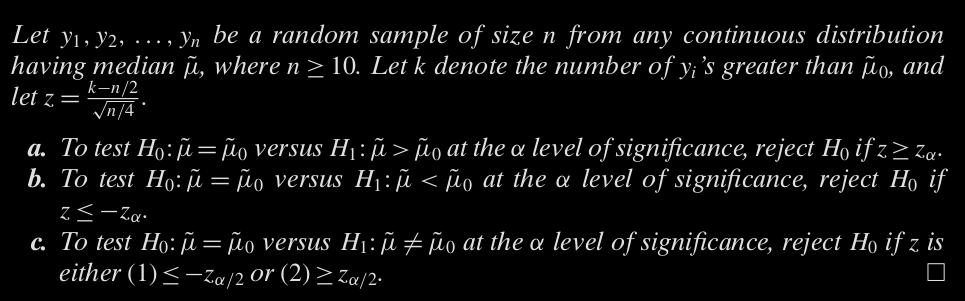
\includegraphics[scale=0.3]{./Codes/SignTest_LargeSample.png}
\end{center}
\bigskip
\bigskip

\item When sample size $n$ is small: use the exact distribution of binomial distribution.
\end{itemize}
\end{frame}
%-------------- end slide -------------------------------%}}}
%-------------- start slide -------------------------------%{{{ 1
\begin{frame}[fragile]
\begin{itemize}
	\item[E.g.1] In a healthy adults, the median pH for synovial fluid is $7.39$.
	\item[] A random sample of $n=43$ is chosen and test
		\begin{align*}
			H_0: \widetilde{\mu}=7.39\quad\text{vs}\quad
			H_0: \widetilde{\mu}\ne 7.39,\qquad \text{at $\alpha=0.10$.}
		\end{align*}
		\begin{center}
			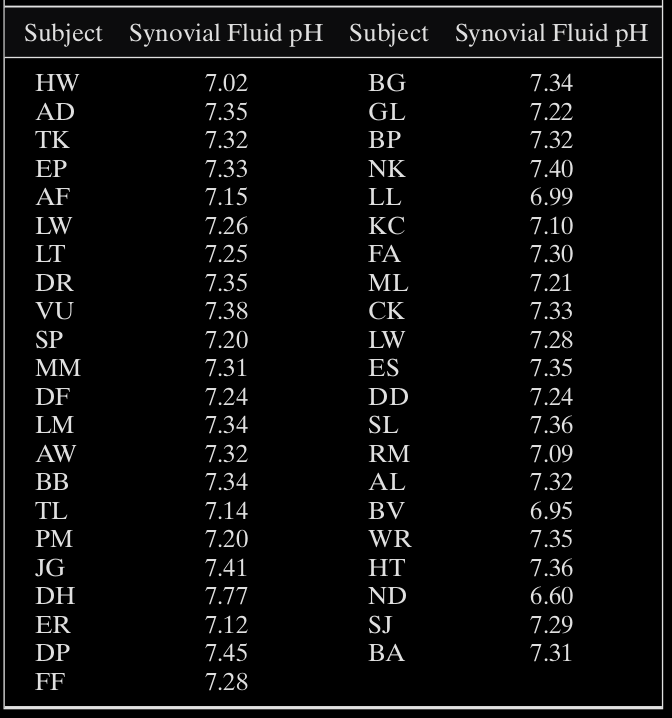
\includegraphics[scale=0.25]{./Codes/Table14-2-1.png}
		\end{center}
\end{itemize}
\end{frame}
%-------------- end slide -------------------------------%}}}
%-------------- start slide -------------------------------%{{{ 1
\begin{frame}[fragile]
\begin{itemize}
	\item[Sol 1.] We first count how many samples exceeding the median (i.e., obtain the value of $X$)
	\begin{center}
		\begin{tikzpicture}[scale=1, transform shape]
			\node (fig) at (0,0) {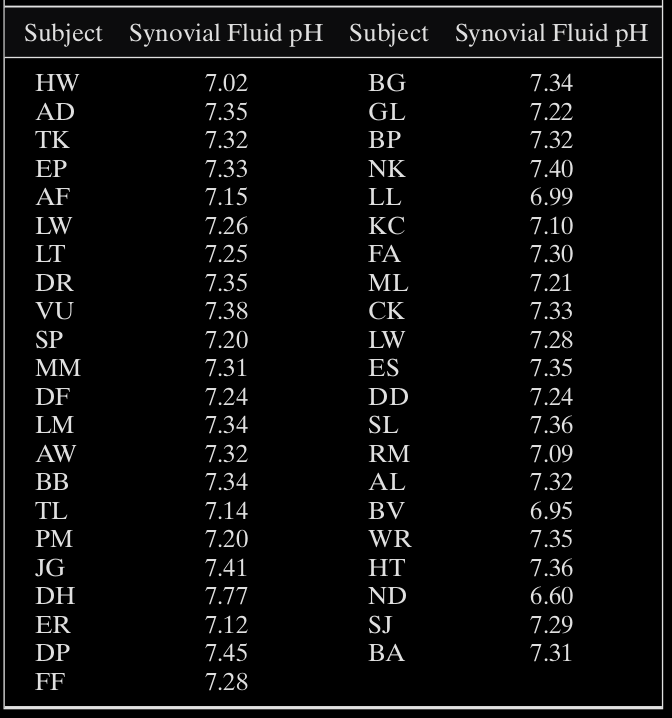
\includegraphics[scale=0.25]{./Codes/Table14-2-1.png}};
			\draw[red] (-1.5,-1.95) rectangle ++(1,0.22) node [right] {$1$};
			\pause
			\draw[red] (-1.5,-2.2) rectangle ++(1,0.22) node [right] {$2$};
			\pause
			\draw[red] (-1.5,-2.7) rectangle ++(1,0.22) node [right] {$3$};
			\pause
			\draw[red] (1.4,1.58) rectangle ++(1,0.22) node [right] {$4$};
		\end{tikzpicture}
	\end{center}
\end{itemize}
\end{frame}
%-------------- end slide -------------------------------%}}}
%-------------- start slide -------------------------------%{{{ 1
\begin{frame}[fragile]
\begin{itemize}
	\item[] Hence, we have $k=4$,  $n=43$, and since $n$ is large, we use the z test:
	\begin{align*}
		z= \frac{4-43/2}{\sqrt{43/4}} = -5.34.
	\end{align*}
	\bigskip

	\item[] Since the critical regions (two-sided test here) are
	\begin{gather*}
		(-\infty,-z_{\alpha/2}) \cup (z_{\alpha/2},\infty)\\ || \\
		(-\infty,-2.58) \cup (2.58,\infty),
 	\end{gather*}
	\item[] we reject the hypothesis.
	\bigskip
	\item[] Or equivalently, the p-value is
	\begin{align*}
		2\times \bbP(Z<-5.34) = 9.294658\times 10^{-8}.
	\end{align*}
	\myQED
\end{itemize}

\mySeparateLine
\vspace{-1.5em}
\begin{center}
\begin{minipage}{0.65\textwidth}
\begin{lstlisting}
> pnorm(-5.34) *2
[1] 9.294658e-08
\end{lstlisting}
\end{minipage}
\end{center}
\end{frame}
%-------------- end slide -------------------------------%}}}
%-------------- start slide -------------------------------%{{{ 1
\begin{frame}[fragile]
\begin{itemize}
	\item[Sol 2.] We can also carry out the exact computation thanks to computer:
	\item[] The exact p-value should be
	\begin{align*}
		2\times\bbP(X\le 5) = 2 \sum_{k=0}^5 \binom{43}{k}\left(\frac{1}{2}\right)^{43} = 2.49951\times 10^{-7},
	\end{align*}
	which is smaller than $\alpha=0.10$.
	\item[] Hence, rejection! \myQED
\end{itemize}
\vfill

\mySeparateLine
\vspace{-1.5em}
\begin{center}
\begin{minipage}{0.65\textwidth}
\begin{lstlisting}
> pbinom(5,43,0.5) * 2
[1] 2.49951e-07
\end{lstlisting}
\end{minipage}
\end{center}

\end{frame}
%-------------- end slide -------------------------------%}}}
%-------------- start slide -------------------------------%{{{ 1
\begin{frame}[fragile]
	\frametitle{Sign test for paired data}
	\begin{itemize}
		\item[E.g.] A manufacturer produces two products, A and B. The manufacturer wishes to know if consumers prefer product B over product A.
		\item[] A sample of 10 consumers are each given product A and product B, and asked which product they prefer:\\
		\begin{center}
				\begin{tabular}{c|c}
				\renewcommand{\arraystretch}{2}
				Preferences   & Number \\
				\hline
				B             & 8 \\
				A             & 1 \\
				No preference & 1 \\
				\end{tabular}
		\end{center}
		\bigskip
	\item[] Test at $\alpha=0.10$ that
	\begin{gather*}
		\text{$H_0$: consumers do not prefer B over A}\\
		\text{vs.}\\
		\text{$H_1$: consumers do prefer B over A}.
	\end{gather*}
	\end{itemize}
\end{frame}
%-------------- end slide -------------------------------%}}}
%-------------- start slide -------------------------------%{{{ 1
\begin{frame}[fragile]
\begin{itemize}
	\item[Sol.] We first remove the ties. So that we have a random (paired-data) sample of size $n=9$.
	\bigskip

	\item[] Under $H_0$, the consumers have no preference for B over A. Hence, we may believe that consumers will choose A or B with probability $\frac{1}{2}$.
	\bigskip

	\item[] Hence, to get more extreme values in this setting would give the p-value:
	\begin{align*}
		\bbP(X\ge 8) = \sum_{k=8}^9 \binom{9}{k} \left(\frac{1}{2}\right)^{9} = 0.0195.
	\end{align*}
	\bigskip

	\item[] Conclusion, Rejection! \myQED
\end{itemize}
\end{frame}
%-------------- end slide -------------------------------%}}}
